\documentclass[12pt]{article}
 \usepackage[utf8]{inputenc}
   \usepackage[slovene]{babel}
\usepackage{amsthm, amsfonts, amsmath, amssymb, url}
\usepackage{graphicx}
\usepackage{subfigure}

\textheight 210 true mm
\textwidth 146 true mm
\voffset=-17mm
\hoffset=-13mm


\begin{document}

\thispagestyle{empty}
\begin{center}
\begin{Large}
{\bf N-kotna ``biljardna'' miza}
\end{Large}
\\[5mm]
\begin{large}
Poročilo za projekt pri {\em matematično modeliranje}
\\[5mm]
{\sc Matej Čušin}
\\[10mm]
28. 5. 2021
\end{large}

\end{center}

\newpage
\setcounter{page}{1}
\noindent
\section{Razvoj projekta}

Pri predmetu matematočno modeliranje smo za zaključek predmeta dobili vsak svoj projekt, ki ga je potrebno razrešiti s pomočjo Matlaba.\\



\subsection{Navodilo naloge}

``Biljardna" miza ima obliko pravilnega $n$-kotnika. Iz neke točke na mizi pošljemo kroglico proti sredini prve stene. Odbije se po odbojen zakonu, kjer je trk prožen in se vsa energija ohrani. Trenje zanemarimo. Napišite program, ki izriše animacijo $k$ odbojev kroglice. Če problema ne znate rešiti splošno, ga poskusite obravnavati vsaj za $n = 4$ in nekaj odbojev.

\subsection{Kako smo razrešili}

Najprej smo napisali dodatno funkcijo, ki je določila koordinate oglišč pravilnega $n$-kotnika. Središče tega $n$-kotnika se nahaja na koordinatah $[r, r]$ zato, da se lažje poišče naključno točko za začetek. Na koncu smo ugotovili, da je za sode $n$ primeren $n$-kotnik, kjer se ``prvo" oglišče nahaja na koordinatah $[2r, r]$. Izkaže se, da pri lihih tak $n$-kotnik ni primeren, ker je imela ena stranica koeficient $\infty$. Zato smo potem lihe $n$-kotnike obrnili za $\frac{\pi}{2}$ v pozitivno smer (nasprotna smer kot urin kazalec), torej pri lihih $n$-kotnikih se ``prvo" oglišče, nahaja na koordinatah $[r, 2r]$. \\
Nato smo iz teh točk sestavili poligon z ukazom v Matlabu $polyshape$. Nato smo ustvarili naključno točko znotraj tega poligona in jo usmerili proti središču prve stranice. Prva stranica pri sodih $n$-kotnikih je tista, ki ima za rob oglišče v $[2r, r]$ in se nadaljuje v pozitivni smeri, pri lihih $n$-kotnikih je tista, ki ima za rob oglišče v $[r, 2r]$ in se nadaljuje v pozitivni smeri.\\
Potem pa program poskrbi za odboj v pravo smer in  poišče novo točko odboja. Poskrbi tudi za animacijo, kako kroglica potuje.

\newpage

\section{Kako ustvariti aplikacijo}

\subsection{GUI Matlab}
\begin{flushleft}
	Na začetku se moramo postaviti v Matlabu v \textbf{appdesigner}. To storimo tako, kot kaže spodnja slika.
\end{flushleft}
	

\centering
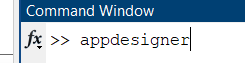
\includegraphics{app1.png}
\linebreak


\begin{flushleft}
	V \textbf{appdesignerju} se nam ponudi več predlog za GUI, mi smo uporabili \textbf{Blank App}.
\end{flushleft}

\centering
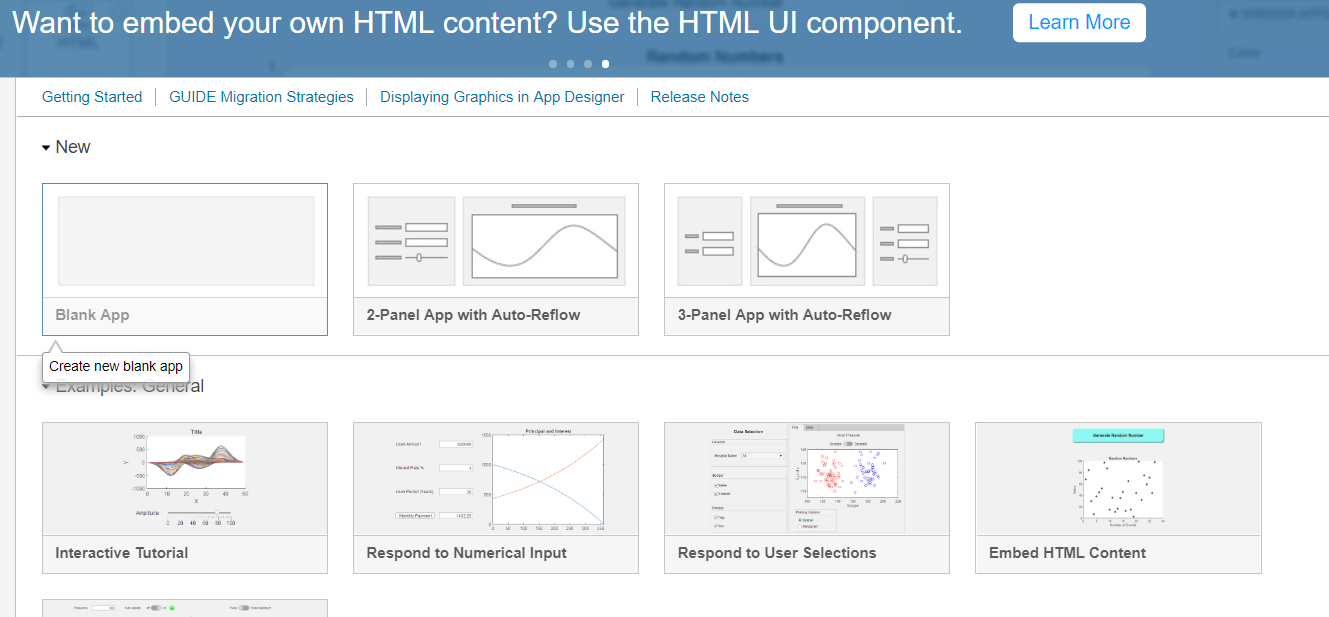
\includegraphics[scale=0.70]{app2.png}
	
\begin{flushleft}
	Sedaj pa le ustvarimo ustrezen vmesnik, kot ga želimo, in dobimo $.mlapp$ datoteko.
\end{flushleft}

\subsection{Ustvariti EXE datoteko}

\begin{flushleft}
	Najprej moramo zagnati \textbf{Application Compiler}, to storimo tako:
\end{flushleft}

\centering

\includegraphics{app3.png}
\linebreak

\centering
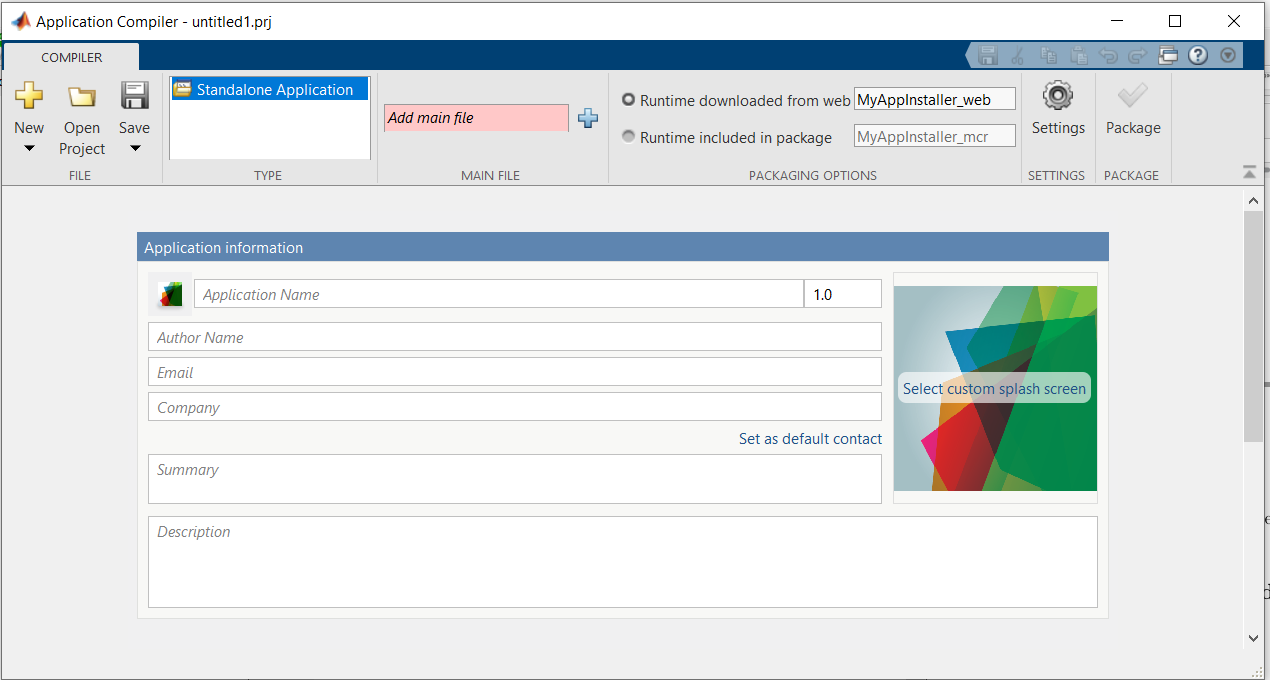
\includegraphics[scale=0.70]{app4.png}	
\linebreak

\begin{flushleft}
	V \emph{Add main file} dodamo $mlapp$ datoteko, ki smo jo generirali na prejšnem koraku. Poimenujemo jo tako, kot želimo, da bi bilo ime naši aplikaciji, nato pa zgolj pritisnemo \textbf{Package} in se nam ustvari imenik:
\end{flushleft}


\centering
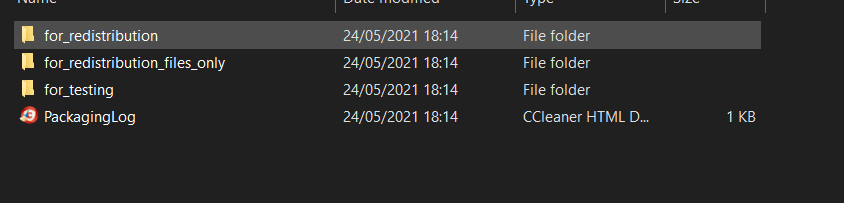
\includegraphics{app5.png}



\begin{flushleft}
	V imeniku \textbf{for\_redistribuition} se nahaja $.exe$ datoteka, ki zažene aplikacijo za namestitev le te aplikacije na računalniku. V drugih dveh pa ustvari $.exe$ datoteko, ki zažene aplikacijo (zagon traja kar nekaj časa).\\
	Ko se aplikacija zažene, nam ponudi dve polji, da vpišemo željeni $n$ (kakšen $n$-kotnik) in $k$ (število odbojev). Ko pritisnemo na gumb \textbf{Start}, se zažene animacija. Ko se prva animacija zaključi, lahko nastavimo druge parametre. Ko pritisnemo na gumb \textbf{Start}, program spet izbere naključno točko in izvede odboje.
\end{flushleft}

\centering
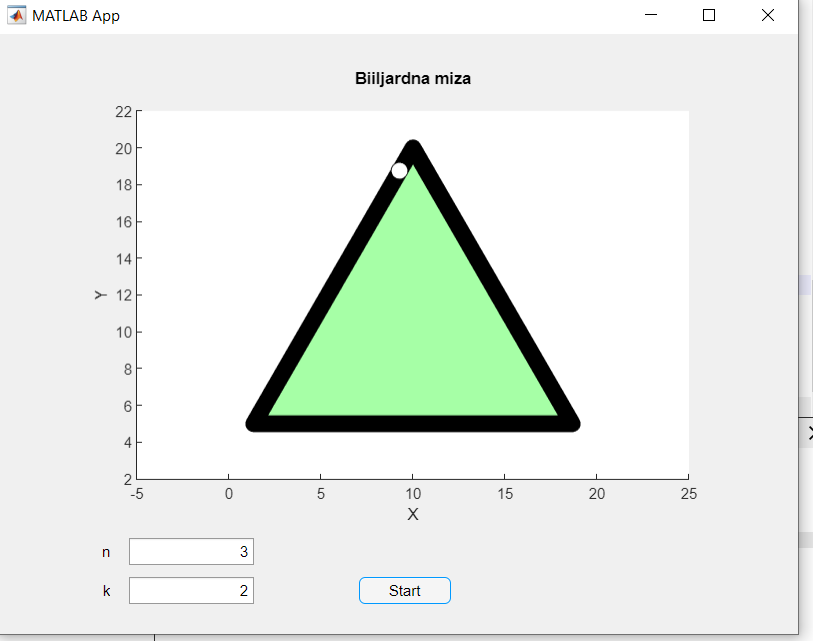
\includegraphics[scale=0.85]{app6.png}
\newpage	

\section{Splošno}

\begin{flushleft}
	Prilagoditev velikosti $n$-kotnika lahko nastavimo zgolj v $projekt.m$. V aplikaciji se velikosti, ne da bi posegli v kodo, ne da spremeniti.\\
	Tukaj lahko tudi vidimo pot kroglice, to uredimo tako, da v $51$ vrstici odstranimo komentar. S tem lahko potem tudi preverimo, da kroglica ostane znotraj $n$-kotnika, seveda zakomentiramo animacijo.\\
	Spodaj sta dve sliki, ko je $k$=100, za pravilni 6-kotnik in pravilni 3-kotnik.
\end{flushleft}


\begin{figure}[!htb]
	\centering
	\subfigure[]{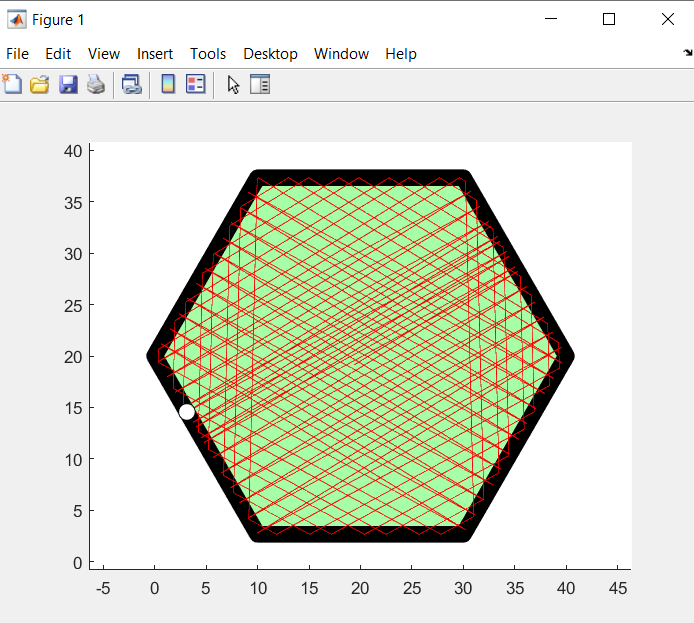
\includegraphics[width=0.45\textwidth]{slikaSod.png}} 
	\subfigure[]{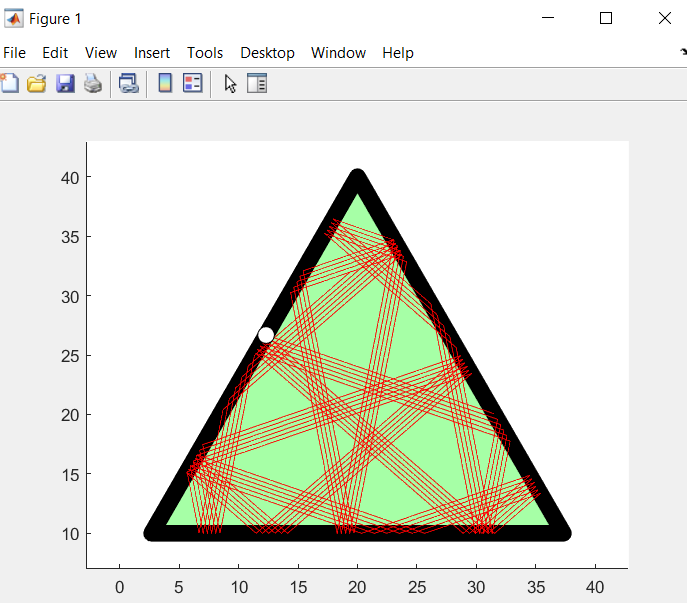
\includegraphics[width=0.45\textwidth]{slikaLih.png}}
	\caption{(a) 6-kotnik (b) 3-kotnik}
\end{figure}	

\subsection{Razporeditev datotek}

\begin{itemize}
	\item
	Običajne Matlab datoteke:
	\begin{itemize}
		\item
		projekt.m - program, ki poskrbi za pravilnost in število odbojev,
		\item
		n\_kotnik.m - program, ki poskrbi za ustvarjanje pravilnega $n$-kotnika.
	\end{itemize}
	\item
	Programi za aplikacijo:
	\begin{itemize}
		\item
		projektApp.mlapp - program, ki sestavi ustrezen GUI,
		\item
		Aplikacija - imenik, ki ga ustvari Matlab med tem, ko za $mlapp$ datoteko ustvari $exe$ datoteko.
	\end{itemize}
	\item
	Datoteke za poročilo:
	\begin{itemize}
		\item
		slike, ki so v poročilu,
		\item
		datoteke, ki ji Latex ustvari sam.
	\end{itemize}
\end{itemize}

\subsection{Viri}

\begin{itemize}
	\item
	Matlab dokumentacija.
	\item
	Avtor - youtube račun - Civil Engineering and programming (7. 8. 2019). CONVERT MATLAB GUI INTO APPLICATION(.EXE EXTENSION) [Video]. Pridobljeno s \url{https://www.youtube.com/watch?v=n9Y1_8jsvVkr} (ogled: 25. 5. 2021).
	\item
	Avtor - youtube račun - MATLAB (23. 1. 2018). Building MATLAB Apps with App Designer [Video]. Pridobljeno s \url{https://www.youtube.com/watch?v=nQb0qBiDurU} (ogled: 25. 5. 2021).
\end{itemize}

\end{document}

